%-------------------------------------------------------------------------------
%	CAPITOLO 43
%-------------------------------------------------------------------------------

\chapter{Capitoli mai scritti}
Nel retro dell'ultimo quaderno ho trovato alcuni appunti e titoli di capitoli  a matita che Mingazzi non è mai riuscito a scrivere. Vi riporto le annotazioni:\\
\\\emph{Ed ecco Alessandrino dei miei Natali\\
Coi suoi coniughi e le cubicazioni\\
Che per virtù di cappe e di piviali\\
Divenne anche Assessor dei matrimoni
\\\index[Personaggi]{Natali Alessandro (assessore)}
\rule{1.5cm}{0.4pt}\\
\\
Don \index[Personaggi]{Don Servidei Serafino}Servidei\footnote{Don Serafino Servidei fu il parroco presente durante la settimana rossa ad Alfonsine}
\\
\rule{1.5cm}{0.4pt}\\
\\
Il Santo
\\
\rule{1.5cm}{0.4pt}\\
\\
\index[Personaggi]{Fabbri Cesare}Fabbri Cesare (ricordi funebri (cavallo))}\\\\

\newpage

\noindent In allegato vi era anche questo appunto:\\

\noindent \emph{Casa posta sulla via\\
elta o basa che lì sia\\
quant cla pies e su patron\\
cusavut te e mi cuion}\\
\begin{figure}[hbt]
\begin{center}
\vspace{-10pt}
   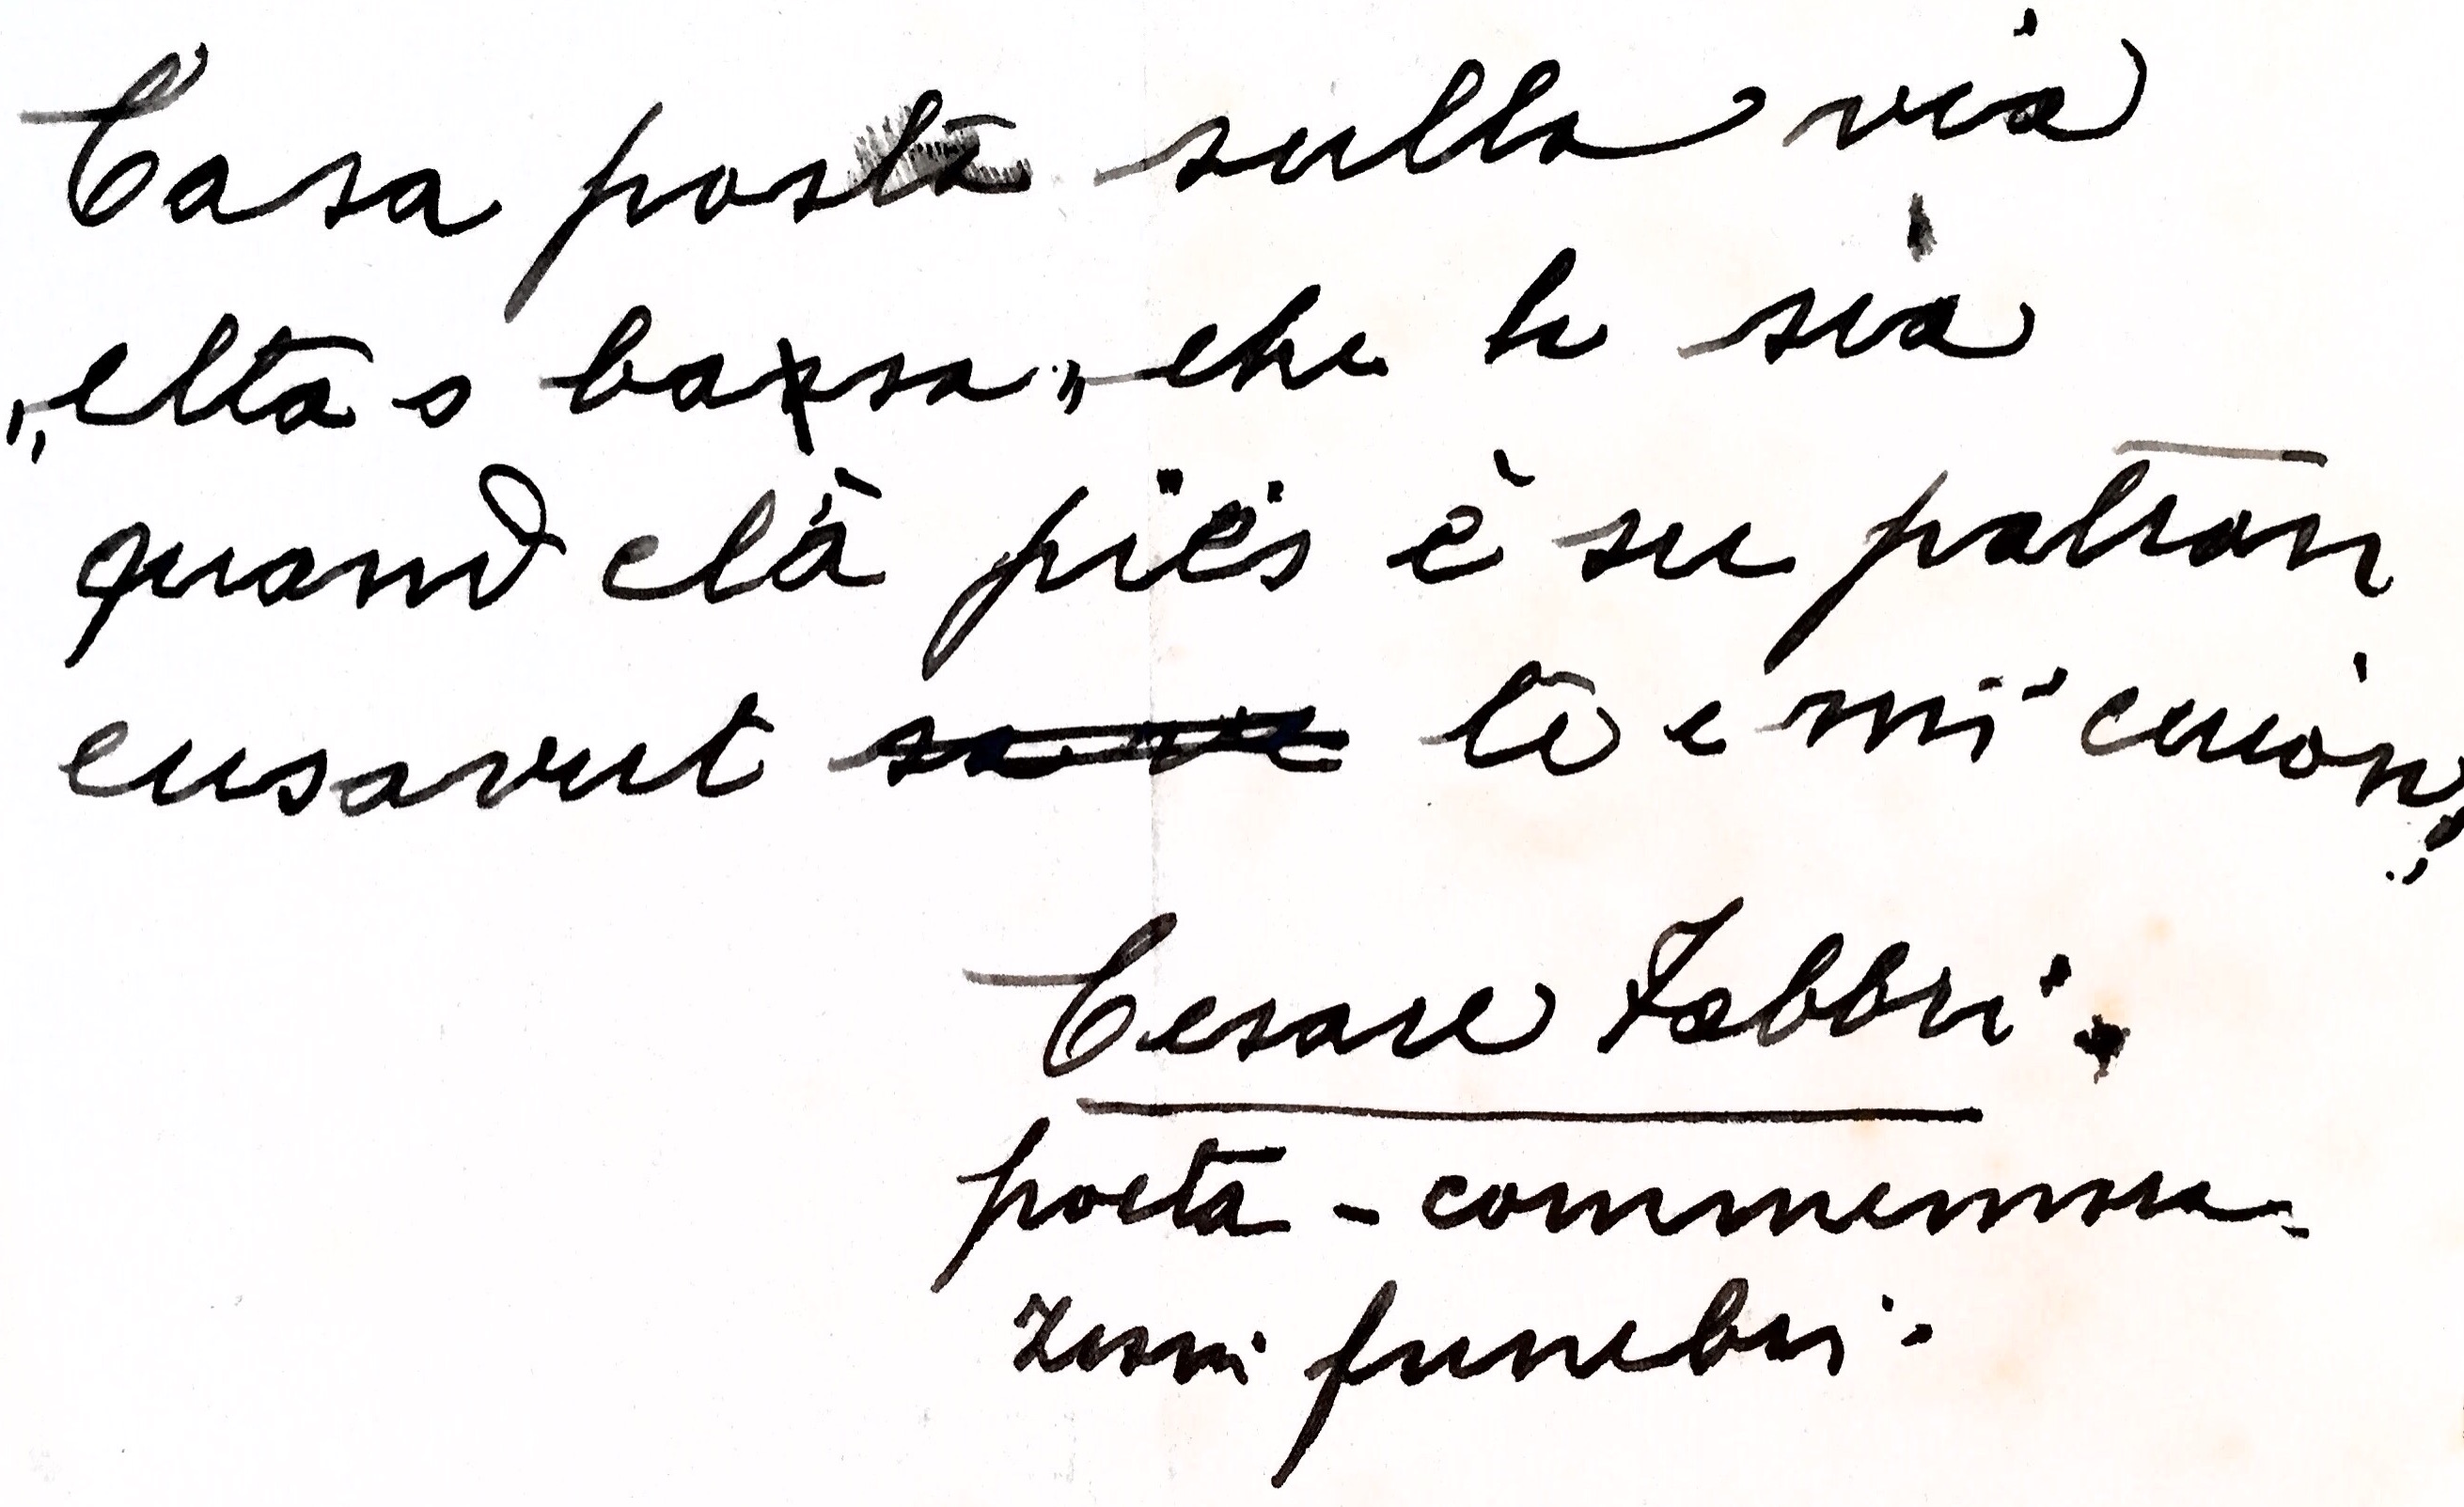
\includegraphics[width=\textwidth]{FabbriCesare}
  \end{center}
\end{figure}

\rule{1.5cm}{0.4pt}\\
\\
\emph{Don \index[Personaggi]{Don Battista}Battista (è proibito friggere nella padella, la signora E. M. rise: "io friggerò in una casseruola")}



